%
% fvm.tex
%
% (c) 2020 Prof Dr Andreas Müller, Hochschule Rapperswi
%
\section{Finite Volumina
\label{section:finite-volumina}}
\rhead{Finite Volumina}
Die Diskretisierung mit Hilfe eines Gitters hat auf Variablen $u_{ik}$
geführt, die Werte der Funktion $u$ an den Gitterpunkten waren.
Die Werte der Funktion zwischen diesen Punkten haben für die
diskretisierten Gleichungen keine Rolle gespielt.
Ausserdem hat sich gezeigt, dass Gleichungen erster Ordnung
nur mit Kompromissen auf diese Weise diskretisiert werden.

Am Beispiel der zweidimensionalen Kontinuitätsgleichung soll
in diesem Abschnitt illustriert werden, wie die gleiche Information,
die in der Differentialgleichung steckt, auch in einer Integralform
dargestellt werden kann.
Dies führt auf eine alternative Diskretisation, in der wir nicht
auf Differenzenquotienten angewiesen sind.

\subsection{Die Kontinuitätsgleichung}
Die Kontinuitätsgleichung beschreibt die Tatsache, dass in einem
strömenden Fluid Materie nicht einfach aus dem Nichts entstehen kann
oder verschwinden kann.
Sie stellt eine Beziehung her zwischen der Dichte $\varrho$ und der
Strömungsgeschwindigkeit $v$.
Der Einfachheit halber untersuchen wir das Problem nur in einer
Dimension.
Die Dichte $\varrho(x,t)$ wie auch die Geschwindigkeit $v(x,t)$
ist eine Funktion von Ort und Zeit.

Zur Herleitung der Kontinuitätsgleichung betrachten wir ein
Interval $[x,x+\Delta x]$.
Zur Zeit $t$ enthält es ungefähr die Masse $\varrho(x,t)\cdot\Delta x$.
Die Masse kann sich während eines Zeitintervals $\Delta t$ dadurch
ändern, dass Materie durch das linke und rechte Intervallende strömt.
Die Menge, die durch das rechte Ende strömt ist
$\varrho(x+\Delta x,t)\cdot v(x+\Delta x,t)\cdot \Delta t$,
durch das linke Ende strömt
$\varrho(x,t)\cdot v(x,t)\cdot \Delta t$.
Die Masseänderung ist die Differenz, also
\[
\varrho(x+\Delta x,t)\cdot v(x+\Delta x,t)\cdot \Delta t
-
\varrho(x,t)\cdot v(x,t)\cdot \Delta t
=
\varrho(x,t+\Delta t)\Delta x
\varrho(x,t)\Delta x.
\]
Nach Division durch $\Delta t\Delta x $ bleibt die Gleichung
\[
\frac{\varrho(x+\Delta x,t)v(x+\Delta x,t) - \varrho(x,t)v(x,t)}{\Delta x}
=
\frac{\varrho(x,t+\Delta t)-\varrho(x,t)}{\Delta t}.
\]
Im Grenzwert $\Delta t\to 0$ un d$\Delta x\to 0$ entsteht die
die partielle Differentialgleichung
\begin{equation}
\frac{\partial (\varrho v)}{\partial x} = \frac{\partial \varrho}{\partial t}
\qquad\Leftrightarrow\qquad
\frac{\partial\varrho}{\partial t} - \frac{\partial j}{\partial x}=0,
\label{pde:eqn:kontinuitaetsgleichung}
\end{equation}
wobei wir in der letzten Umformung $j=\varrho v$ für den Massefluss
geschrieben haben.
Die Gleichung \eqref{pde:eqn:kontinuitaetsgleichung} heisst die
{\em Kontinuitätsgleichung}.
\index{Kontinuitätsgleichung}%

Die Kontinuitätsgleichung kann ganz analog auch in höheren Dimensionen
hergeleitet werden.
Für den Stromvektor $\vec{\jmath}=\varrho\vec{v}$ gilt
\[
\frac{\partial \varrho}{\partial t}
-
\operatorname{div}(\varrho \vec{v})
=
\frac{\partial \varrho}{\partial t}
-
\operatorname{div}\vec{\jmath}
=
0,
\]
wobei die {\em Divergenz}
\index{Divergenz}%
eines Vektorfeldes $\vec{a}$ durch
\[
\operatorname{div}\vec{a}
=
\frac{\partial a_x}{\partial x}
+
\frac{\partial a_y}{\partial y}
+
\frac{\partial a_z}{\partial z}
\]
gegeben ist.

\subsection{Integralform}
Die Herleitung der Kontinuitätsgleichung basiert auf dem Vergleich
von Funktionswerten von $\varrho$ und $j$ in den Eckpunkten eines
Rechtecks mit Kantenlänge $\Delta x$ und $\Delta t$ in der $x$-$t$-Ebene.
Alternativ hätten wir aber auch Integrale entlang der Kanten verwenden
können, um die Veränderung der Masse im Interval $[x,x+\Delta x]$ 
zu berechnen.

Die Masse im Interval $[x,x+\Delta x]$ ist gegeben durch das Integral
\[
m(t) = \int_x^{x+\Delta x} \varrho(\xi, t) \,d\xi
\]
der Dichte über das Interval.
Die Änderung der Masse zwischen den Zeiten $t$ und $t+\Delta t$ entsteht
durch den Fluss durch die Endpunkte.
Durch den linken und rechten Endpunkt des Intervalls fliesst im Zeitinterval
$[t,t+\Delta t]$ die Masse
\[
\int_t^{t+\Delta t} j(x,\tau)\,d\tau
\qquad\text{bzw.}\qquad
\int_t^{t+\Delta t} j(x+\Delta x,\tau)\,d\tau.
\]
Änderiung der Masse zwischen den Zeitpunkten $t$ und $t+\Delta t$
ist die Differenz, also
\begin{align}
m(t+\Delta t)-m(t)
&=
\int_t^{t+\Delta t}j(x+\Delta x,\tau)\,d\tau
-
\int_t^{t+\Delta t}j(x,\tau)\,d\tau
\notag
\\
\Rightarrow\qquad
\int_x^{x+\Delta x} \varrho(\xi,t+\Delta t)\,d\xi
-
\int_x^{x+\Delta x} \varrho(\xi,t)\,d\xi
&=
\int_t^{t+\Delta t}j(x+\Delta x,\tau)\,d\tau
-
\int_t^{t+\Delta t}j(x,\tau)\,d\tau
\label{pde:eqn:integralform}
\end{align}
Diese Gleichung gilt für beliebig grosse Schritte $\Delta x$ und
$\Delta t$, sie ist also nicht nur eine Approximation wie die
Differenzenquotienten, die für die Herleitung der Kontinuitätsgleichung
verwendet wurden. 
Die Differenzenquotienten ergaben erst im Grenzwert eine exakte
Gleichung.
Wir nennen 
\eqref{pde:eqn:integralform}
die Integralform der Kontinuitätsgleichung.

Die Herleitung der Integralform lässt sich auch in der mehrdimensionalen
Situation durchführen.
Dazu muss man einerseits die Masse $m(t)$ in einem Volumn $V$ berechnen,
was mit dem Dreifachintegral
\[
m(t)
=
\iiint_V \varrho(x,y,z,t) \,dV
\]
geschehen kann.
Andererseits muss man den Materiefluss durch die Oberfläche von $V$
berechnen können, was das Flussintegral
\[
\oint_{\partial V} \vec{\jmath}(x,y,z,t) \,d\vec{n}
\]
tut.
Die Integralform der Kontinuitätsgleichung wird damit
\[
\iiint_V \varrho(x,y,z,t+\Delta t) \,dV
-
\iiint_V \varrho(x,y,z,t) \,dV
=
\oint_{\partial V} \vec{\jmath}(x,y,z,t+\Delta t)\,d\vec{n}
-
\oint_{\partial V} \vec{\jmath}(x,y,z,t)\,d\vec{n}.
\]


\subsection{Diskretisation}
\begin{figure}
\centering
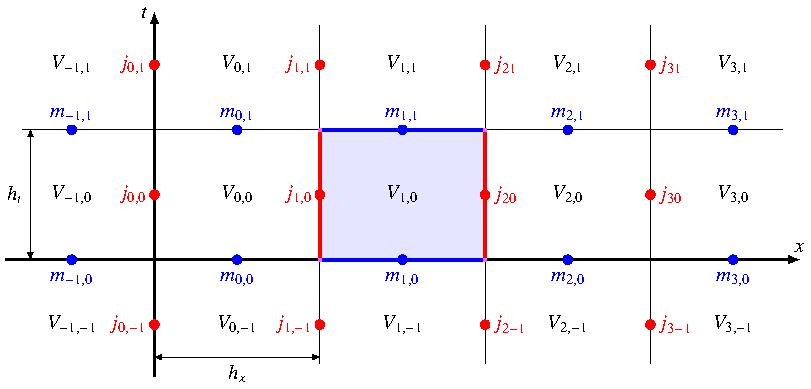
\includegraphics{chapters/70-pde/images/kont.pdf}
\caption{Diskretisation der Kontinuitätsgleichung~\eqref{pde:fvm:1dim}
mit Hilfe diskreter Volumina. 
Die Variablen $m_{ik}$ stehen für die im Interval $[ih_x,(i+1)h_x]$
enthaltene Masse, $j_{ik}$ steht für die im Zeitinterval $[kh_t,(k+1)h_t]$
durch das Intervallende $ih_x$ fliessende Masse.
\label{buch:pde:fvdisk}}
\end{figure}
Die Integralform~\eqref{pde:eqn:integralform}
der Kontinuitätsgleichung suggeriert, dass die Integrale
in dieser Gleichung bessere Variablen für eine Diskretisation
sein könnten.

Wir verwenden wieder ein Gitter in der $x$-$t$-Ebene, aber 
als gesuchte Variablen verwenden wir Integrale
\begin{align*}
m_{ik}
&=
\int_{ih_x}^{(i+1)h_x} \varrho(\xi,kh_t)\,d\xi
\\
j_{ik}
&=
\int_{kh_t}^{(k+1)h_t} j(ih_x,\tau) \,d\tau
\end{align*}
der Funktionen über Kanten im Gitter, wie in Abbildung~\ref{buch:pde:fvdisk}
dargestellt.
Die Kontinuitätsgleichung wird damit zu
\begin{equation}
m_{i,k+1}-m_{ik}
=
j_{i+1,k}-j_{ik}.
\label{pde:fvm:1dim}
\end{equation}
Man beachte auch hier wieder, dass dies keine Approximation ist, sondern
dass diese Gleichungen exakt gelten.

Um diese Idee auf höhere Dimensionen zu verallgemeinern zerlegt man
das Gebiet in kleine Volumina $V_i$.
Die Variablen
\[
m_{ik} = \int_{V_i} \varrho(x, kh_t)\, dV
\]
berechnen die Masse, die im Volumen $V_i$ enhalten sind.
Die Masseänderung in einem Zeitintervall setzt sich aus den
Masseflüssen durch die verschiedenen Seitenflächen $V_i$ 
zusammen.
Seien $\sigma_{il}$ die Seitenflächen des Volumens $V_i$
Daher verwenden wir 
\[
j_{ilk} = \int_{\sigma_{il}} \vec{\jmath}\,(\xi, kh_t)\,d\vec{n}.
\]
Für jedes Volumen nimmt die Kontinuitätsgleichung die Form
\begin{equation}
m_{i,k+1}-m_{ik}
=
\sum_{\text{$l$ Seitenfläche von $V_i$}} (j_{il,k+1}-j_{ilk}).
\label{pde:fvm:ndim}
\end{equation}
an.
Wieder sind lineare Gleichungen entstanden.
Haben zwei Volumina $V_{i_1}$ und $V_{i_2}$ die Seite
$\sigma_{i_1j_1}=\sigma_{i_2j_2}$ gemeinsam, dann sind die 
zugehörigen Flüsse entgegengesetzt:
\[
j_{i_1l_1k}=j_{i_2l_2k}
\qquad\forall k\in\mathbb Z,
\]
denn was das Volumen $V_{i_1}$ durch die Seite $\sigma_{i_1l_1}$ an
Masse verliergt gewinnt das Volumn $V_{i_2}$ durch die Seite
$\sigma_{i_2l_2}$.

Die Gleichungen \eqref{pde:fvm:1dim} und \eqref{pde:fvm:ndim} für
sich alleine können reichen nicht, weitere Gleichungen wie die
Navier-Stokes-Gleichung werden zusätzlich benötigt, um ein Strömungsfeld
vollständig zu beschreiben.
Es ist allerdings nicht das Ziel dieses Abschnitts, die Methode
der {\em finiten Volumina} in voller Allgemeinheit zu entwickeln.





